\subsection*{Общая характеристика работы}


\newcommand{\contribution}{{\textbf{Личный вклад автора в публикации с соавторами.}}}

{\actuality}
Обзор, введение в тему, обозначение места данной работы в мировых исследованиях и~т.\:п.

 \aim\ данной работы является \ldots

Для~достижения поставленной цели необходимо было решить следующие {\tasks}:
\begin{enumerate}
  \item Исследовать, разработать, вычислить и~т.\:д. и~т.\:п.
  \item Исследовать, разработать, вычислить и~т.\:д. и~т.\:п.
  \item Исследовать, разработать, вычислить и~т.\:д. и~т.\:п.
  \item Исследовать, разработать, вычислить и~т.\:д. и~т.\:п.
\end{enumerate}

\defpositions
\begin{enumerate}
  \item Первое положение
  \item Второе положение
  \item Третье положение
  \item Четвертое положение
\end{enumerate}

\novelty
\begin{enumerate}
  \item Впервые \ldots
  \item Впервые \ldots
  \item Было выполнено оригинальное исследование \ldots
\end{enumerate}

\influence\ \ldots

\reliability\ полученных результатов обеспечивается \ldots \ Результаты находятся в соответствии с результатами, полученными другими авторами.

\probation\
Основные результаты работы докладывались~на:
перечисление основных конференций, симпозиумов и~т.\:п.

\contribution\ Автор принимал активное участие \ldots

\publications\ Основные результаты по теме диссертации изложены в 8 печатных изданиях~\cite{skalko2014, tsybulin2015a, tsybulin2015b},
2 из которых изданы в журналах, рекомендованных ВАК~\cite{skalko2014,tsybulin2015a}, 
5 --- в тезисах докладов~\cite{miptconf53,miptconf54,miptconf55,miptconf56,miptconf57}.
 % Характеристика работы по структуре во введении и в автореферате не отличается (ГОСТ Р 7.0.11, пункты 5.3.1 и 9.2.1), потому её загружаем из одного и того же внешнего файла, предварительно задав форму выделения некоторым параметрам

\newcommand{\epar}[1]{\underline{\textbf{#1}}}

%\newpage
\subsection*{Основное содержание работы}
\textbf{Объём и структура работы.} Диссертация состоит из~введения, пяти глав, заключения, списка литературы и двух приложений. Полный объём диссертации составляет 112 страниц
с~38 рисунками и 3 таблицами. Список литературы содержит 51 наименование.

Во \epar{введении} обосновывается актуальность исследований, проводимых в рамках данной диссертационной работы, формулируется цель, ставятся задачи работы, сформулированы научная новизна, теоретическая и практическая значимость представляемой работы, описаны методология и методы исследования, обоснована достоверность представленных результатов. Приведен обзор существующих методов решения уравнения переноса.

% ================================================================

\subsubsection*{Первая глава}
В \epar{первом параграфе} описывается математическая модель процесса переноса излучения. 
В работе рассматривается стационарное уравнение переноса для функции интенсивности излучения
$I(\mathbf r, \boldsymbol \Omega)$, 
\[
(\boldsymbol \Omega  \nabla) I + \varkappa(\mathbf r) I(\mathbf r, \boldsymbol \Omega) = \varkappa(\mathbf r) I_\text{p}(\mathbf r),
\]
которое справедливо в предположении отсутствия рассеяния и переизлучения на других частотах. Уравнение выражает баланс лучистой энергии, заключенной в элементарном объёме окружающем луч $\mathbf r - \mathbf r_0 = \boldsymbol \Omega s$. Приводятся несколько типов граничных условий для уравнения переноса излучения. Показана роль излучения в системе уравнений радиационной газовой динамики. 

Во \epar{втором параграфе} приводится самосопряженная форма уравнения переноса излучения и ее слабая постановка, полученная из вариационного принципа Владимирова. 

В \epar{третьем параграфе} приводится многогрупповая локально термодинамически равновесная модель поглощения излучения околозвездным веществом, состоящим из атомов и ионов водорода. В модели учитывается доплеровский сдвиг частоты поглощения при прохождении излучения через движущееся вещество. При вычислении коэффициента поглощения в спектральной линии используется тот факт, что интегральный по частоте коэффициент поглощения одного атома не зависит от ширины линии, а лишь от квантово-механических характеристик перехода атома между состояниями $n$ и $n'$:
\[
\int\limits_{-\infty}^\infty \varkappa_\nu d\nu = N \vartheta_n \int\limits_0^\infty \sigma_\nu d\nu = N \vartheta_n \frac{\pi e^2}{m_e c} f_{nn'}.
\]
Здесь $\varkappa_\nu$ --- коэффициент поглощения на частоте $\nu$, $\sigma_\nu$ --- сечение рассеяния, $\vartheta_n$ --- доля атомов, находящихся в состоянии $n$, $N$ --- концентрация атомов, $f_{nn'}$ --- сила осциллятора для перехода $n \to n'$. Для вычисления доли $\theta_n$ использовалось ионизационное уравнение Саха
\[
\frac{(\alpha^+)^2}{1 - \alpha^+} = 2 \frac{u^+}{u_0} \frac{m_p }{\rho\Lambda^3} \exp\left(-\frac{\epsilon}{kT}\right),
\]
где $\alpha^+$ --- доля ионов водорода, $u^+, u_0$ --- электронные статистические суммы для иона и нейтрального атома, $\Lambda$ --- тепловая дебройлевская длина волны электрона, $\epsilon$ --- энергия ионизации атома.

% ================================================================

\subsubsection*{Вторая глава}
%\subsubsection*{Третья глава}
Посвящена построению метода на основе вариационного принципа для задачи переноса излучения. В \epar{первом параграфе} изложен метод Ритца для данной вариационной постановки. Метод Ритца используется для дискретизации как пространственной, так и угловой зависимости решения. В качестве пространственного базиса используются кусочно-линейные непрерывные функции, а для угловой части рассмотрен базис из сферических функций (классический метод сферических гармоник) и базис из радиальных функций
\[
R_i(\boldsymbol \Omega) = \exp (-\epsilon_i ||\boldsymbol \Omega - \boldsymbol \omega_i||^2) + \exp (-\epsilon_i ||\boldsymbol \Omega + \boldsymbol \omega_i||^2).
\]

\epar{Второй и третий параграфы} посвящены выводу квадратурных формул для упрощенного вычисления объемных и поверхностных интегралов. Для вычисления интегралов по угловой переменной на сфере предлагается использовать квадратурные формулы Лебедева. Для вычисления интегралов на границе области требуется проводить интегрирование
\[
\iint\limits_{(\boldsymbol \Omega \mathbf n) < 0}  Q(\boldsymbol \Omega)\: (\boldsymbol \Omega \mathbf n) d\Omega
\]
по полусфере направлений, содержащихся в области. Описывается подход к построению такой квадратурной формулы. 

В \epar{четвертом параграфе} рассматривается метод сопряженных градиентов для решения линейной системы и предлагается метод диагонального углового предобуславливания для случая базиса сферических функций. Каждая операция предобуславливания эквивалентна решению набора независимых скалярных уравнений эллиптического типа с операторами вида
\[
\mathcal{L}\varphi = -\div \frac{\operatorname{diag}(c_1, c_2, c_3)}{\varkappa}\grad \varphi + \varkappa \varphi,
\]
где среди чисел $c_1, c_2, c_3$ не более двух различных. Аналогичное предобуславливание производится и для метода с радиальными базисными функциями.

В \epar{пятом параграфе} приводится способ восстановления физических величин плотности энергии излучения, потока энергии излучения и тензора потока импульса излучения по четным угловым моментам функции интенсивности.

В \epar{шестом параграфе} приведены особенности реализации данного метода с использованием графических ускорителей. Рассматривается вопрос о компактном представлении вспомогательных матриц и структуры расчетной сетки.

% ================================================================

\subsubsection*{Третья глава}
%\subsubsection*{Четвертая глава}
Приводится описание маршевого метода для уравнения переноса излучения. В \epar{первом параграфе} демонстрируется, как применение метода коротких характеристик и разрывного метода Галеркина приводят к необходимости упорядочения элементов расчетной сетки.

Во \epar{втором параграфе} рассматриваются способы повышения порядка аппроксимации метода коротких характеристик путем увеличения количества узловых точек в тетраэдре. На примере равномерной прямоугольной сетки показывается, что множество узловых точек с необходимостью должно содержать вершины сеточного элемента. В случае нарушения данного условия, излучение в численном решении не распространятся под углами $0 < \theta < \theta_\text{кр}$ к сторонам прямоугольника (см. рисунок \ref{fig:instab}), а сам метод теряет устойчивость.
\begin{figure}[ht!]
\centering
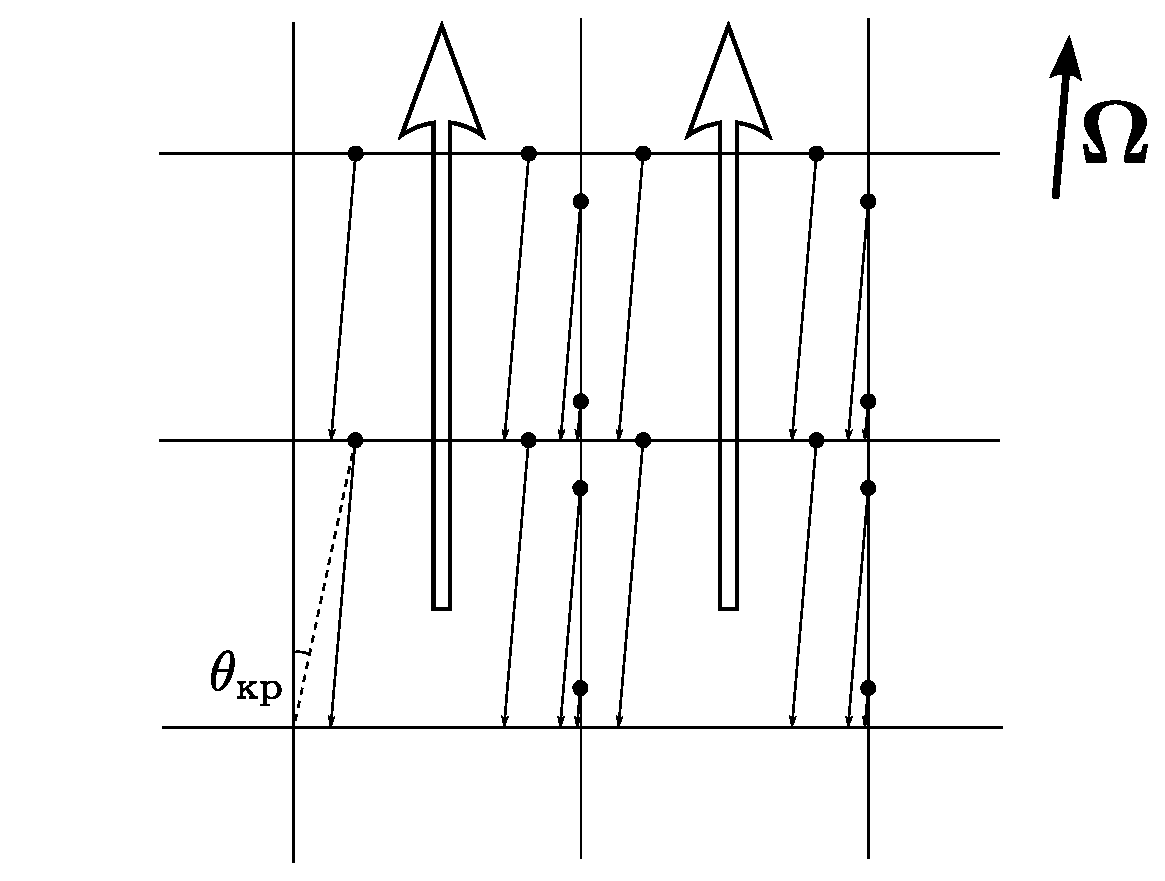
\includegraphics[height=.25\textheight]{instab.eps}
\caption{Направление распространения излучения в численной схеме (контурная стрелка) и истинное направление $\boldsymbol \Omega$ в случае нарушения условия размещения узлов (точки) на сторонах прямоугольной сетки}
\label{fig:instab}
\end{figure}

В качестве дополнительных узлов для метода второго порядка предлагается использовать середины ребер тетраэдров. Для обеспечения в схеме монотонности квадратичной интерполяции предложена процедура коррекции значений интенсивности в серединах ребер по следующему правилу:
\[
\tilde I_\text{mid} = \frac{I_1 + I_2}{2} + \operatorname{clamp}\left(
I_\text{mid} - \frac{I_1 + I_2}{2}; \left[
- \frac{|I_2 + I_1|}{4}, \frac{|I_2 + I_1|}{4}
\right]
\right),
\]
где $I_1, I_2$ --- значения интенсивности в концах ребра, $I_\text{mid}$ --- значение интенсивности в середине ребра, полученное до монотонизации, $\tilde I_\text{mid}$ --- значение после монотонизации, $\operatorname{clamp}(x, [a, b]) \equiv \max(a, \min(b, x))$.

\epar{Третий параграф} содержит изложение двух алгоритмов упорядочения элементов сетки. Первый алгоритм упорядочивает тетраэдры согласно проекции центра их описанной сферы на направление излучения $\boldsymbol \Omega$. Приводится доказательство корректности данного алгоритма в случае, когда сетка удовлетворяет условию Делоне. Предложен алгоритм упорядочения тетраэдральной сетки общего вида, основанный на модификации алгоритма поиска в ширину.

В \epar{четвертом параграфе} показана связь между ярусно-параллельной формой алгоритма вычисления решения и отношением частичного порядка, полученным после упорядочения элементов сетки.

% ================================================================

\subsubsection*{Четвертая глава}
%\subsubsection*{Пятая глава}
Рассматривается распределенный метод длинных характеристик. В \epar{первом параграфе} изложена идея стандартного метода длинных характеристик. 
Продемонстрировано, что для коэффициентов $\alpha(s, s_0), \beta(s, s_0)$, используемых для компактного выражения оператора Грина задачи переноса излучения
\[
I(\mathbf r_0 + \boldsymbol \Omega s, \boldsymbol \Omega) = 
\alpha(0, s) I(\mathbf r_0, \boldsymbol \Omega) + \beta(0, s),
\]
справедливо \emph{трассировочное соотношение}
\[\begin{aligned}
\alpha(s_0, s) &= \alpha(s_0, s_1) \alpha(s_1, s),\\
\beta(s_0, s) &= \beta(s_0, s_1) \alpha(s_1, s) + \beta(s_1, s),
\end{aligned}
\]
где точка $\mathbf r_0 + \boldsymbol \Omega s_1$ расположена на луче между $\mathbf r_0 + \boldsymbol \Omega s_0$ и $\mathbf r_0 + \boldsymbol \Omega s$, см. рисунок~\ref{fig:trace}. Данное соотношение крайне удобно, так как позволяет вычислить $\alpha(0, s)$ и $\beta(0, s)$, последовательно проходя по сеточным элементам от конца луча к началу.
\begin{figure}[ht!]
\centering
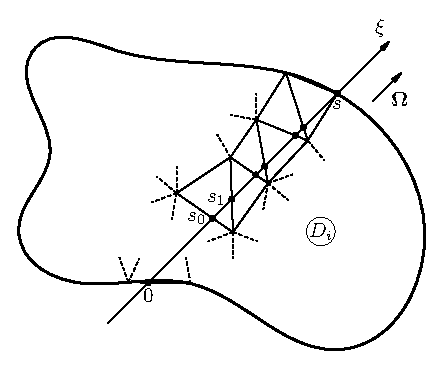
\includegraphics[height=.2\textheight]{trace-0.eps}
\caption{Трассировка луча от точки $\xi = s$ до точки $\xi = 0$}
\label{fig:trace}
\end{figure}

Во \epar{втором параграфе} вводится понятие входной, выходной и касательной к направлению излучения грани тетраэдра. Если $\mathbf n$ --- нормаль к грани, а $\boldsymbol \Omega$ --- направление излучения, то в случае
%\newpage
\begin{itemize}
\item если $(\mathbf n \boldsymbol \Omega) < -\epsilon$, то грань называется входной (луч входит в тетраэдр);
\item если $(\mathbf n \boldsymbol \Omega) > \phantom{-}\epsilon$, то грань называется выходной (луч выходит из тетраэдра);
\item иначе, грань называется касательной.
\end{itemize}
В этом определении $\epsilon \ll 1$ --- малое число, позволяющее различить входные и выходные грани устойчиво к ошибкам округлений. Доказывается 
\emph{лемма об устойчивой трассировке}, в которой утверждается, что луч, проходящий через точку $Q$ в многограннике $T$ в направлении $-\boldsymbol \Omega$, гарантированно выйдет через входную (в смысле определения выше) грань при условии, что точка $Q$ находится на расстоянии более $\delta = \epsilon \cdot d(T)$ от каждой грани. Здесь $d(T)$ обозначает диаметр многогранника $T$. Иллюстрация данного условия приведена на рисунке~\ref{fig:shift}.
\begin{figure}[ht!]
\centering
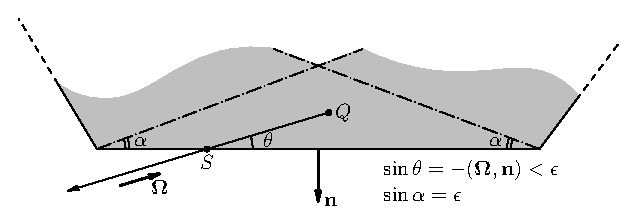
\includegraphics[width=.6\textwidth]{shift-0.eps}
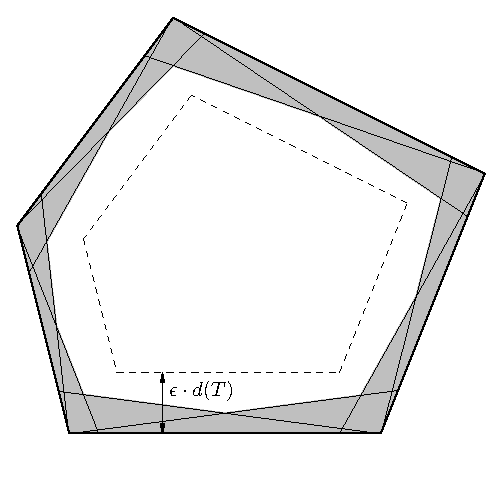
\includegraphics[height=.25\textheight]{shift-1.eps}
\caption{Многогранник $T$, запрещенная область (серая) и гарантированно допустимая область из леммы (пунктир). В трехмерном случае запрещенная область имеет более сложную форму}
\label{fig:shift}
\end{figure}

Чтобы гарантировать условие леммы, при трассировке начальная точка $Q$ смещается внутрь многогранника. Это также решает проблему возможного зацикливания луча при прохождении через вершину, когда из-за ошибок округления точка $Q$ при трассировке через несколько шагов возвращается в тетраэдр, который был уже пройден. При использовании смещения точки $Q$, она гарантированно сдвигается хотя бы на $\epsilon^2 d(T)$ в направлении $-\boldsymbol \Omega$. Для работы алгоритма требуется, чтобы пунктирная область на рисунке~\ref{fig:shift} была непуста, что накладывает определенные ограничения на качество расчетной сетки.

В \epar{третьем параграфе} изложена идея распределенного метода длинных характеристик. Вместо того, чтобы выпускать характеристику из точки $\mathbf r$ до пересечения с границей расчетной области, характеристика выпускается лишь до границы расчетной \emph{подобласти}. Такая характеристика не позволяет найти решение в точке, из которой была выпущена, но позволяет линейным образом связать интенсивность в точке $\mathbf r$ с интенсивностью в основании характеристики $\mathbf r_0$. Поскольку данная точка лежит на границе подобласти, значение интенсивности в ней не известно.

Выпуская характеристики из каждой точки границы подобласти, можно получить набор линейных соотношений, связывающих значения интенсивности на противоположных границах каждой подобласти. Объединяя данные соотношения в единую систему уравнений и дополняя ее граничными условиями, получаем задачу для определения интенсивности на границах расчетных подобластей. Полученная система имеет небольшую размерность, так как в нее входят неизвестные только на границах подобластей, а также преимущественно-треугольный вид при упорядочении неизвестных в зависимости от проекции их координат на направление $\boldsymbol \Omega$. Легко показать диагональное преобладание матрицы данной системы уравнений.

После решения системы линейных уравнений и определения интенсивности на границах подобластей можно провести трассировку внутренних точек каждой подобласти в отдельности. Это действие производится автономно в каждой подобласти.

В \epar{четвертом параграфе} приведены основные особенности параллельной реализации данного алгоритма. Так как решение линейной системы в методе проводится на одном вычислительном узле, для балансировки загрузки узлов предлагается трассировать подобласти по несколько направлений одновременно. При этом для каждого направления полученная система линейных уравнений решается на своем вычислительном узле.

Самым трудоемким этапом работы алгоритма является трассировка внутренних узлов подобластей. Этот этап выполняется с использованием графических ускорителей, причем каждая нить на графическом ускорителе трассирует свой луч. В случае использования нескольких частотных групп, каждая нить трассирует один луч для одной частотной группы.
Показано, что этап коллективного взаимодействия процессов и решения линейных систем можно перекрыть основным этапом вычислений на графических ускорителях, см. временную диаграмму работы алгоритма на рисунке \ref{fig:timeline}.
\begin{figure}[ht!]
\centering
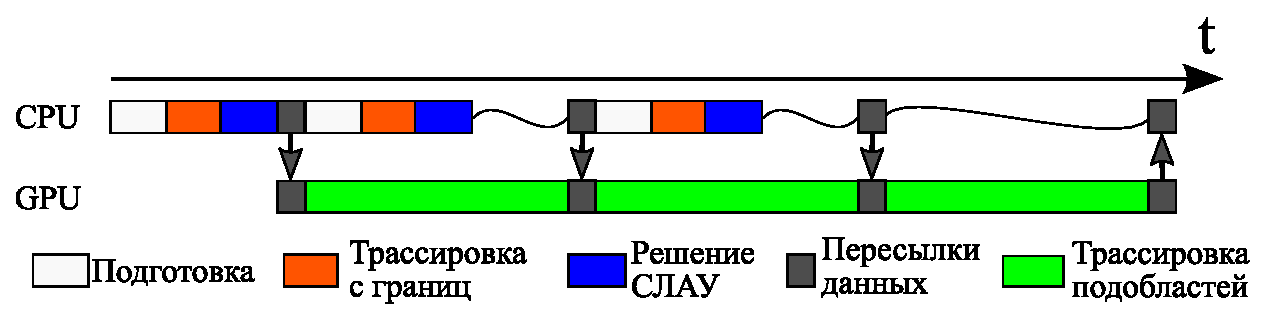
\includegraphics[width=\textwidth]{timeline.eps}
\caption{Временная диаграмма работы распределенного алгоритма метода длинных характеристик}
\label{fig:timeline}
\end{figure}

% ================================================================

\subsubsection*{Пятая глава}
%\subsubsection*{Шестая глава}
В главе содержатся результаты исследования построенных численных методов. В
\epar{первом параграфе} на примере задачи об излучающем оптически плотном шаре
изучается сходимость метода, основанного на вариационном принципе. Использовалось шесть первых приближений метода сферических гармоник (с числом угловых функций $K = 1, 6, 15, 26, 45, 66$ соответственно).
Показано, что в областях гладкости решения пространственная сходимость имеет второй порядок, характерный для используемого метода Ритца. В окрестности границы шара, где коэффициент поглощения скачкообразно меняется и градиент плотности энергии излучения имеет логарифмическую особенность, сходимость по пространственным переменным имеет порядок $0,4$ (см. графики, представленные на рисунке \ref{fig:sphconv}). Порядок сходимости метода в норме $L_2$ по количеству угловых функций составляет $0,29$ ($\varepsilon \sim K^{-0,29}$), см. рисунок \ref{fig:angconv}.
\begin{figure}[ht!]
\centering
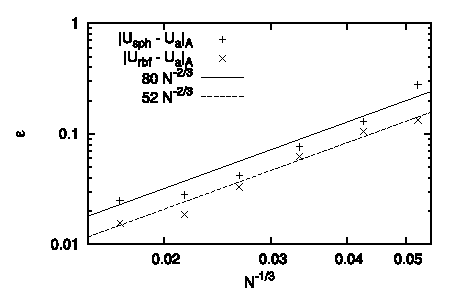
\includegraphics[width=.45\textwidth]{UAerr.eps}
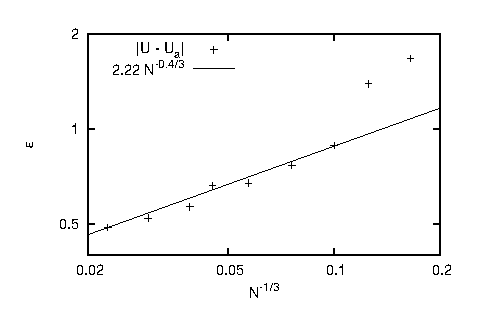
\includegraphics[width=.45\textwidth]{UBerr.eps}
\caption{Ошибка сходимости $\varepsilon$ в центре шара (слева) и на краю шара (справа) в зависимости от мелкости сетки $N^{-1/3}$}
\label{fig:sphconv}
\end{figure}
\begin{figure}[ht!]
\centering
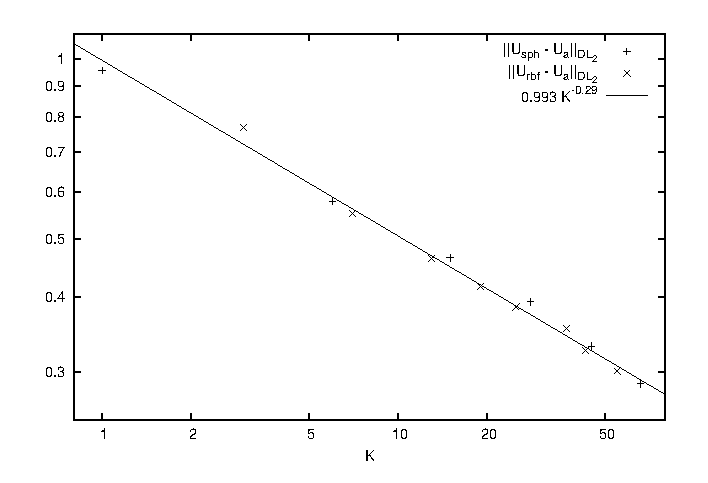
\includegraphics[width=.4\textwidth]{UL2err.eps}
\caption{Ошибка $\varepsilon$ в норме $L_2$ в зависимости от используемого числа угловых функций $K$}
\label{fig:angconv}
\end{figure}

Метод сферических гармоник не обладает <<эффектом луча>>, поскольку линейная оболочка набора сферических функций инвариантна относительно вращений пространства и не содержит выделенных направлений.
Отмечается, что решения, полученные методом сферических гармоник, могут быть нефизичны. Например, тензор направленности излучения (тензор квазидиффузии) $D_{\alpha \beta}$ в задаче об излучающем шаре содержит отрицательные компоненты в областях, удаленных от источника излучения (см. график на рисунке \ref{fig:Drr}, в области, где $D_{rr} > 1$ остальные главные компоненты отрицательны, поскольку $\operatorname{tr} D_{\alpha\beta} = 1$). 
\begin{figure}[ht!]
\centering
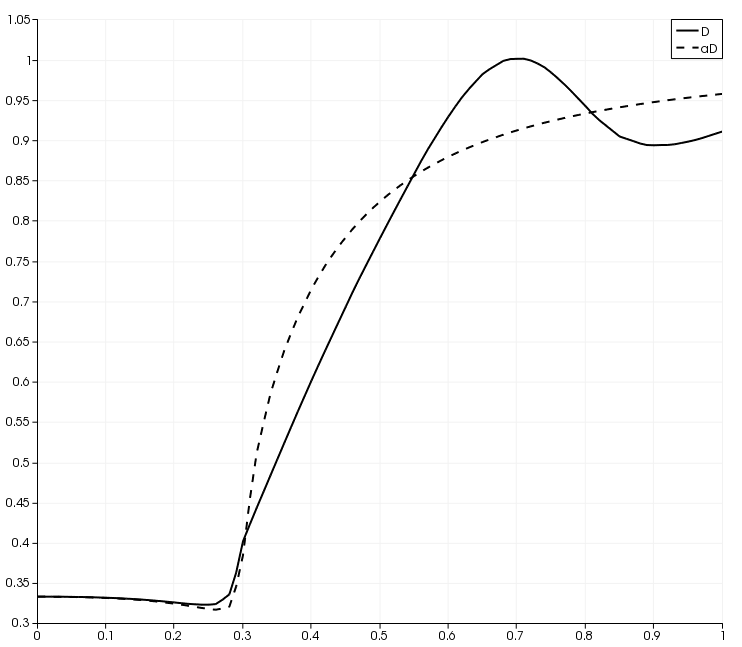
\includegraphics[width=.35\textwidth]{D.png}
\caption{Радиальная компонента тензора направленности излучения $D_{rr}$ в задаче с излучением шара. Пунктиром приведено аналитическое значение}
\label{fig:Drr}
\end{figure}


Метод с базисом из радиальных функций демонстрирует аналогичные результаты сходимости по пространственной переменной, что и метод сферических гармоник. Для этого метода свойственна более быстрая сходимость по числу внешних итераций с предобуславливателем (невязка перестает меняться после $\sim 10$ внешних итераций). Хотя метод имеет выделенные направления, изоповерхности решения сферичны с высокой точностью. Однако, несмотря на то, что все функции радиального базиса строго неотрицательны, коэффициенты разложения численного решения по нему могут оказаться отрицательными. Данное обстоятельство приводит к такому же нефизичному поведению углового распределения интенсивности, что и в методе со сферическими функциями. В целом, данный метод может использоваться как более экономичная альтернатива методу сферических гармоник.

Во \epar{втором параграфе} содержатся результаты решения тестовых задач маршевым методом коротких характеристик. Для исследования эффектов численной диффузии центральное излучающее тело было изменено на оптически плотную область в форме креста, состоящего из 5 равных кубов (см. рисунок \ref{fig:plus}).
На рисунке \ref{fig:march} приведено решение вдоль одного направления, полученное в начале, середине и конце марша.
\begin{figure}[ht!]
\centering
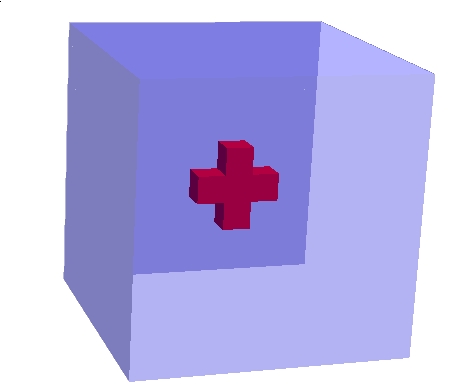
\includegraphics[width=.35\textwidth]{plus.png}
\caption{Вид излучающего тела в задаче для метода коротких характеристик}
\label{fig:plus}
\end{figure}
\begin{figure}[ht!]
\centering
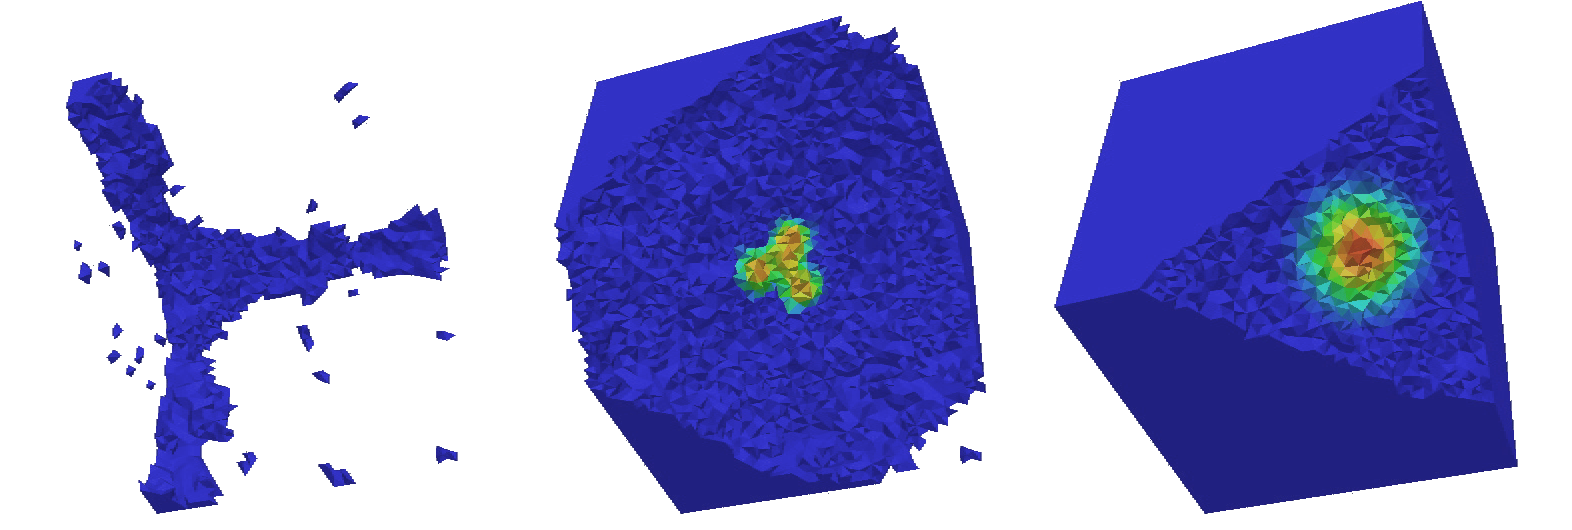
\includegraphics[width=\textwidth]{123.png}
\caption{Решение в различные моменты марша вдоль одного направления. Показаны лишь те элементы, в которых решение уже известно}
\label{fig:march}
\end{figure}

Проведено сравнение методов первого и второго порядка аппроксимации, причем для метода второго порядка рассмотрен вариант без монотонизации и с монотонизацией значения в дополнительных узлах на ребрах тетраэдров (см. рисунок \ref{fig:ord}). В методе второго порядка без монотонизации наблюдаются нефизичные осцилляции амплитудой порядка $20\%$ на границе .
\begin{figure}[ht!]
\centering
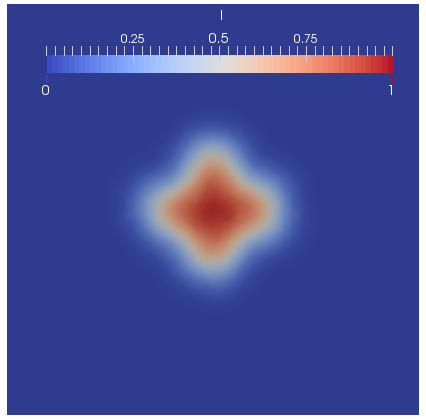
\includegraphics[width=.3\textwidth]{res1ord.png} %
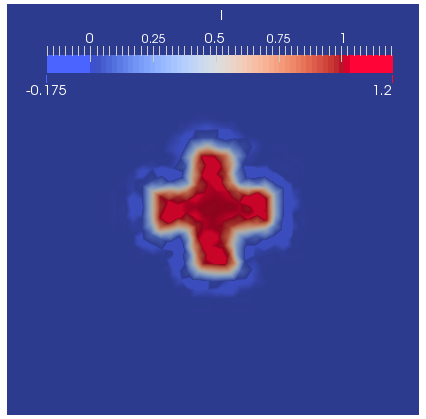
\includegraphics[width=.3\textwidth]{res2nolim.png} %
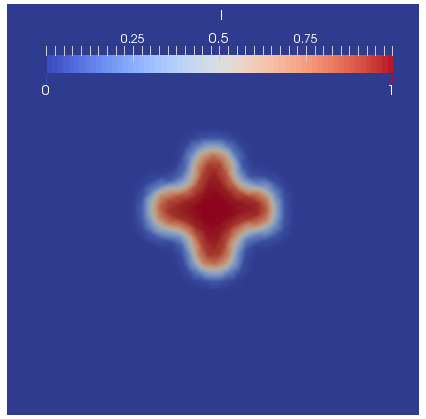
\includegraphics[width=.3\textwidth]{res2wilim.png} %
\caption{Решения вдоль направления к наблюдателю, полученные методами первого порядка, второго порядка и второго порядка с ограничителем}
\label{fig:ord}
\end{figure}

Сравнение плотности излучения показало, что методы первого и второго порядка с ограничителем дают решения, отличающиеся не более чем на $2\%$. В методе второго порядка более выражен <<эффект луча>>, в то время как в методе первого порядка он сглажен численной диффузией лучей.

В \epar{третьем параграфе} приведены результаты исследования распределенного метода длинных характеристик. Отмечено, что численное решение, полученное данным методом, зависит от способа разбиения области на подобласти. Обращается внимание на незначительную численную диффузию луча (см. рисунок \ref{fig:1vs8}), проходящего через границу подобластей, которая существенно меньше, чем в методе коротких характеристик. Значительной диффузии подвержены лишь лучи, проходящие вдоль границы подобластей, но количество таких лучей недостаточно, чтобы существенно повлиять на плотность энергии излучения.
\begin{figure}[ht!]
\centering
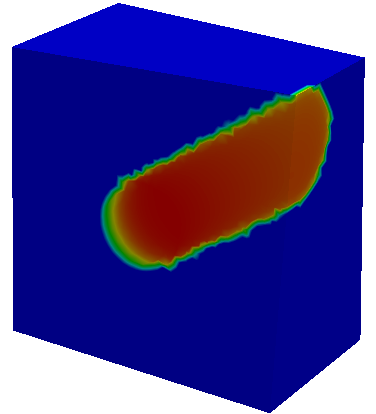
\includegraphics[width=.3\textwidth]{res1piece.png} %
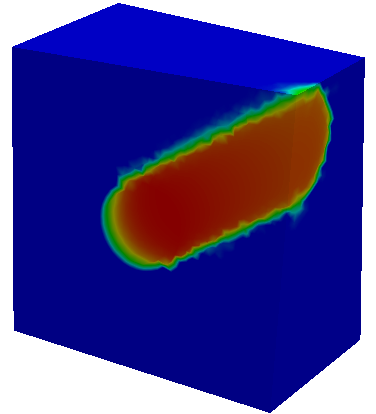
\includegraphics[width=.3\textwidth]{res8pieces.png} %
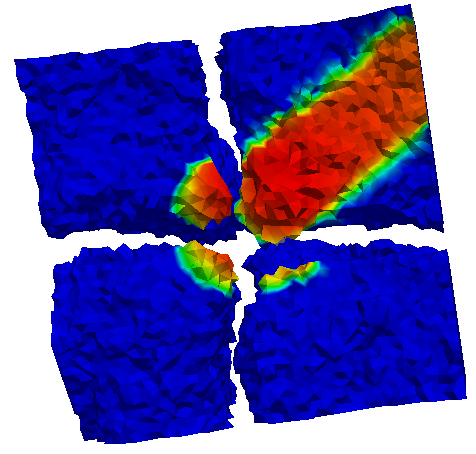
\includegraphics[width=.3\textwidth]{ressplit.png} %
\caption{Решение вдоль одного направления с одной подобластью (слева) и с 8 подобластями (в центре). Справа представлены отдельные подобласти}
\label{fig:1vs8}
\end{figure}

В таблице \ref{tab:speedup} приведено сравнение времени работы алгоритма при
различных разбиениях расчетной области. Данные результаты получены для сетки с
$65 \cdot 10^3$ узлов ($363 \cdot 10^3$ тетраэдров) с использованием $230$ направлений
из квадратурной формулы Лебедева ($25$-й порядок) на высокопроизводительном стенде кафедры информатики и вычислительной математики МФТИ. Незначительное ускорение обусловлено хаотическим доступом к памяти при трассировке лучей, плохой балансировкой нагрузки на графическом ускорителе, а также значительным количеством условных операторов в коде трассировки.
\begin{table}[ht!]
\centering
    \begin{tabular}{|c|c|c|c|c|}
    \hline
    $P$ & Устройства & $t_\text{GPU}, \text{c}$ & $t_\text{CPU}, \text{c}$ & $t_\text{CPU} / t_\text{GPU}$\\\hline
    $1$& 1 x Tesla C2075 & $117$ & $439$ & $3,75$x\\\hline
    $2$& 2 x Tesla C2075 & $52$ & $196$ & $3,77$x\\\hline
    $3$& 3 x Tesla C2075 & $32,7$ & $125$ & $3,82$x\\\hline
    $4$& 3 x Tesla C2075 + GTX 680 & $28,1$ & $108$ & $3,84$x\\
%    $4$& 1 x Tesla C2075 & $88$ & $108$ & $1,23$x\\
	\hline
    $8$& 3 x Tesla C2075 + GTX 680 & $25,5$ & $69$ & $2,70$x\\\hline
    \end{tabular}
\caption{Время работы алгоритма в зависимости от числа подобластей $P$ для MPI реализации (CPU) и MPI+CUDA реализации (GPU)}
\label{tab:speedup}
\end{table}

В \epar{четвертом параграфе} описано использование разработанного метода для расчета спектра
излучения звезды типа Т Тельца, взаимодействующей со своим аккреционным диском.
В определенных условиях такое взаимодействие порождает конический ветер, который
можно обнаружить по синему смещению поглощения в линии H-$\alpha$. В этом расчете вместо квадратурной формулы Лебедева использовалась квазиравномерная угловая сетка из $1091$ направления. Это позволило получить усредненные по периоду обращения звезды спектры при различных углах наклонения $i$ (угол между плоскостью диска и лучом зрения). Использовалось $64$ частотные группы в интервале, соответствующем доплеровскому смещению линии H-$\alpha$ от $-600 \text{ км}/\text{c}$ до $600 \text{ км}/\text{c}$. Зависимость усредненной за период обращения звезды относительной интенсивности $I_\text{o}$ от частоты излучения при разных углах наклонения $i$ представлена на рисунке \ref{fig:spectre}. Для удобства смещение частоты $\Delta \nu$ переведено в относительную скорость $\Delta v = c \frac{\Delta \nu}{\nu_0}$. Можно заключить, что при углах наклонения $i \lesssim 45^\circ$ поглощение в диапазоне синего смещения $\Delta v \sim 150 \dividesymbol 200 \text{ км}/\text{с}$ существенно. Нормализованный профиль линии излучения имеет существенный провал в области красного смещения на скорости $\Delta v \approx 100 \text{ км}/с$, который объясняется значительным поглощением излучения веществом диска, аккрецирующего на звезду.
\begin{figure}[ht!]
\centering
%\includegraphics[width=.45\textwidth]{varinc.eps} %
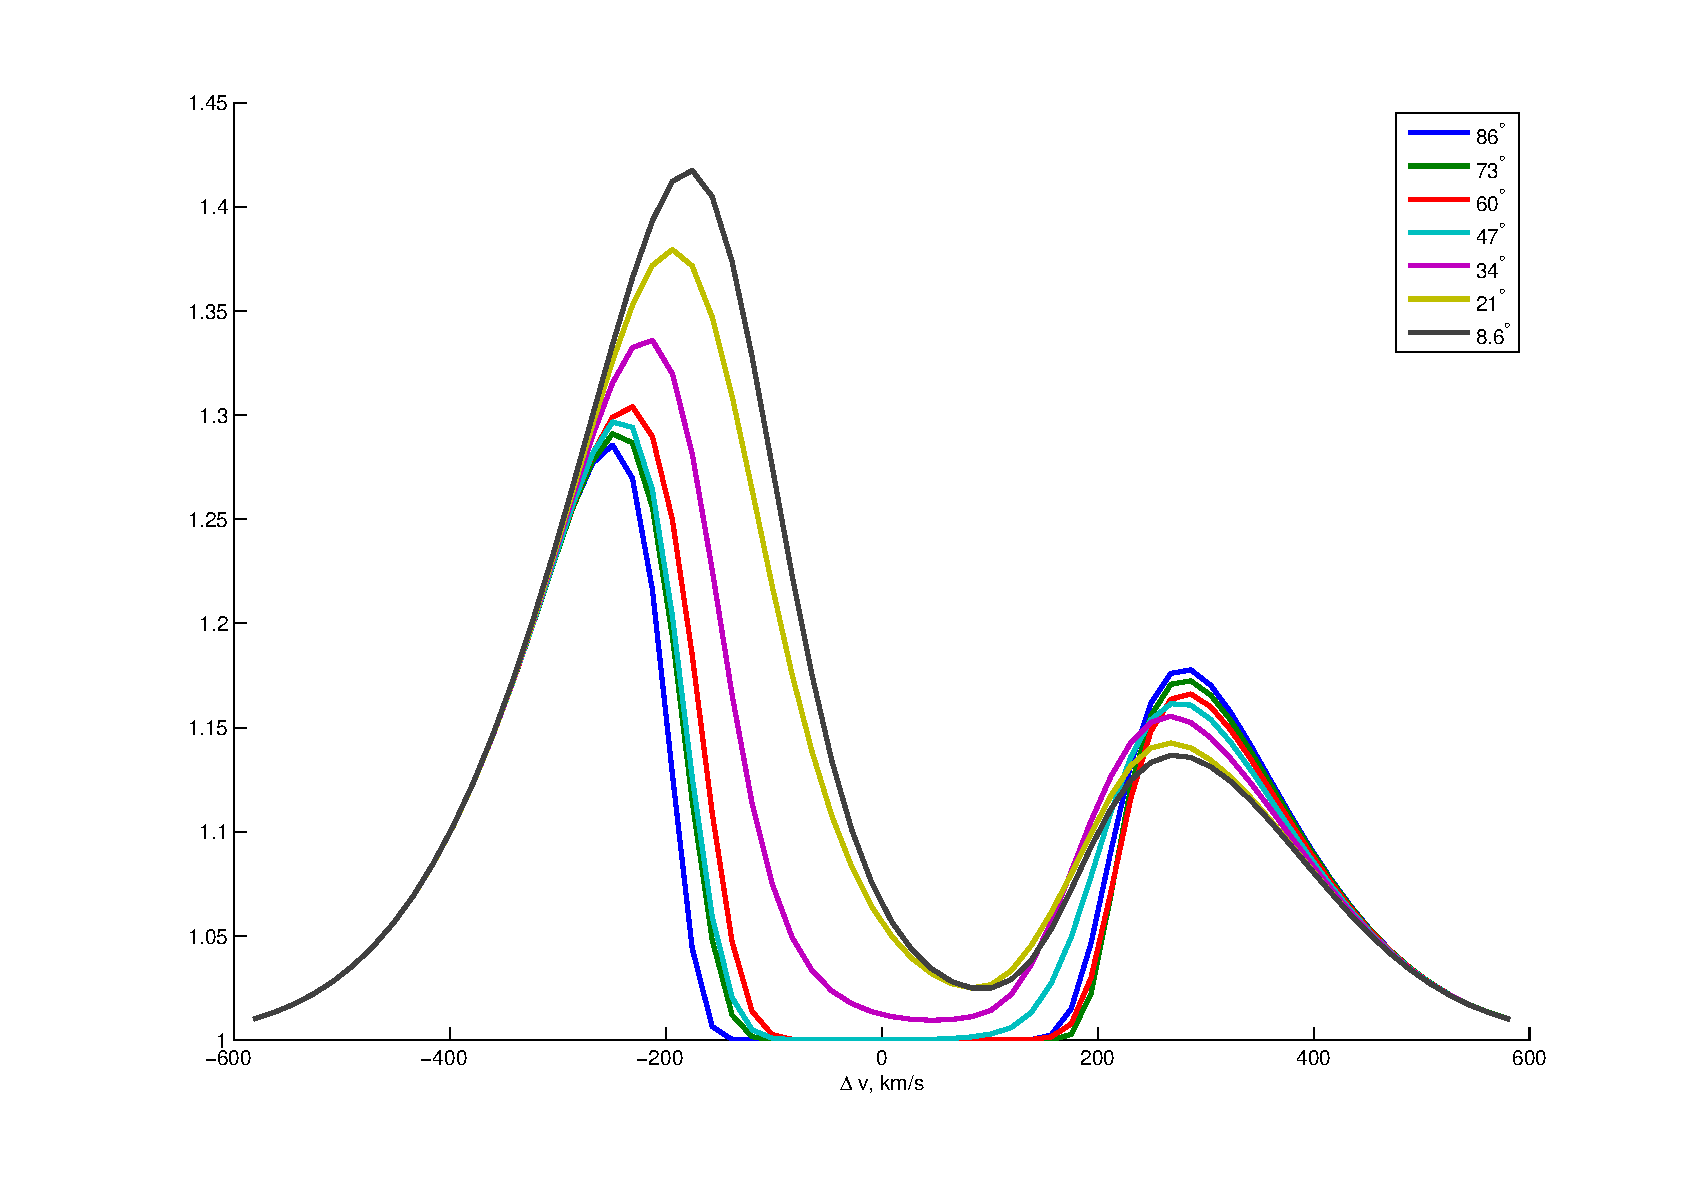
\includegraphics[width=.6\textwidth]{spectrum.eps} %
\caption{Профиль линии H-$\alpha$ в зависимости от угла наклонения $i$}
\label{fig:spectre}
\end{figure}

Для расчета задачи о спектре излучения использовался кластер лаборатории флюидодинамики и сейсмоакустики МФТИ, состоящий из двух узлов, на каждом из которых имеется 8 ускорителей Tesla K40m. На сетке из $5 \cdot 10^5$ узлов (около $3 \cdot 10^6$ тетраэдров) при использовании $110$ направлений и $64$ частотных групп удалось получить ускорение в $4,5$ раза при использовании $16$ графических ускорителей по отношению к MPI реализации с $16$ процессами.

% ================================================================

В \epar{заключении} приведены основные результаты работы.

\subsection*{Основные результаты диссертации}

%% Согласно ГОСТ Р 7.0.11-2011:
%% 5.3.3 В заключении диссертации излагают итоги выполненного исследования, рекомендации, перспективы дальнейшей разработки темы.
%% 9.2.3 В заключении автореферата диссертации излагают итоги данного исследования, рекомендации и перспективы дальнейшей разработки темы.
\begin{enumerate}
  \item Для решения уравнения переноса излучения разработан вариационный метод с радиальными базисными функциями, который обладает точностью, сравнимой с методом сферических гармоник, но при этом более экономичный. Предложенное блочно-диагональное предобуславливание позволяет значительно ускорить вычислительный алгоритм. Построены оптимальные квадратурные формулы для полусферы, инвариантные относительно группы вращений.
  \item Разработан маршевый метод коротких характеристик. Построены варианты метода первого и второго порядка аппроксимации. Получено условие расположения узлов, выполнение которого необходимо для устойчивости метода второго порядка. Для монотонизации схемы второго порядка применен ограничитель значения интенсивности в дополнительных узлах.
  \item Для маршевого метода построены алгоритмы упорядочения неструктурированных сеток. Дополнительным результатом работы алгоритмов упорядочения является ярусно-параллельная форма графа зависимостей вычислительного метода, которую можно использовать для распараллеливания процесса решения задачи. 
  \item Разработана версия метода длинных характеристик, адаптированная для распределенной реализации на многопроцессорных системах и на кластерах с графическими ускорителями. Исследованы ускорение и эффективность реализаций в зависимости от числа используемых вычислительных узлов и графических ускорителей.
  \item Разработанные вычислительные алгоритмы реализованы в программном комплексе. В рамках модели локального термодинамического равновесия вычислен коэффициент поглощения частично ионизованной плазмы. Для задачи моделирования спектра излучения звезды типа Т Тельца построен спектральный профиль линии H-$\alpha$ в зависимости от ориентации плоскости аккреционного диска.
\end{enumerate}


%\newpage
\renewcommand{\refname}{\large Публикации автора по теме диссертации}
\nocite{*}
\insertbiblioauthor                          % Подключаем Bib-базы
%\insertbibliofull

\subsection*{\contribution}
В работе \cite{skalko2014} автором разработан и реализован маршевый метод и алгоритмы упорядочения неструктурированной сетки.

В работе \cite{tsybulin2015a} автор предложил и реализовал распределенный вариант метода длинных характеристик, адаптированный для вычислительного кластера с графическими ускорителями. Автором было проведено исследование ускорения и эффективности параллельной реализации.

В работах \cite{tsybulin2015b, miptconf55, miptconf56, miptconf57, miptconf54} автором построены численные методы для решения уравнения переноса, выполнена алгоритмическая и программная реализация на графических ускорителях методов численного решения систем линейных алгебраических и систем обыкновенных дифференциальных уравнений. Сформулирована задача построения квадратурной формулы для полусферы, которая решена предложенным численным методом продолжения по параметру.
